\ofsubsection{Cerco à Dollet}
%
\ofquote{"O orgulho do Jardim Balamb! A força mercenária de elite, SeeD! Aprenda com eles, obedeça às suas ordens e cumpra a missão. Provem-se dignos de se tornarem um membro da SeeD e boa sorte."}{Diretor Cid}
%
\vfill
%
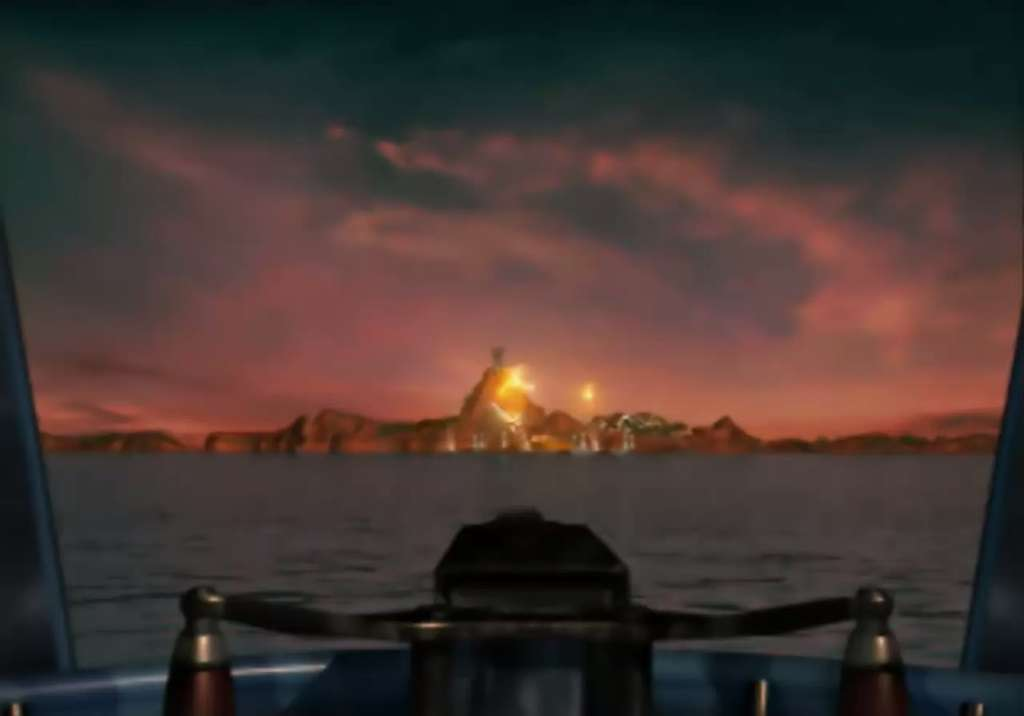
\includegraphics[width=\columnwidth]{./art/siegeofdollet/island.jpg}
%
\vfill
%
\accf{Cerco à Dollet} é uma aventura que pode ser completada em uma única sessão e foi projetada para um grupo de aventureiros de nível~2.
Os jogadores serão estudantes que estão treinando para se tornarem membros de um grupo de mercenários de elite, chamado SeeD.
Você como MJ pode ser o instrutor deles a fim de os guiar através da prova final.
%
\vfill
%
\ofquote{"Parece chato. Então, o que diz é que, façamos todo o trabalhinho sujo..."}{Seifer}
%
\vfill
%
Bom dia, instrutor.
Meu nome é Xu e eu lhe darei tanta informação durante o dia quanto puder.
Você e todos os seus estudantes que farão a prova de hoje deverá ser um de nossas canhoneiras de assalto que estão à caminho de Dollet.
Lembrem-se, o trabalho de vocês é somente guiar os estudantes, não queremos ver se eles podem se provar dignos de se tornarem um SeeD.
Assim sendo, você terá que ficar no barco durante a missão, mas poderá falar com os estudantes a qualquer momento usando um fone de ouvido, pelo qual você também está me ouvindo agora. Certifique-se de que todos saiam com vida!
%
\vfill
%
Quanto a missão:
os esquadrões SeeD foram contratados pelo parlamento de Dollet para os defender contra um cerco do exército de Galbadia.
Seus estudantes forma o esquadrão B e foram incumbidos de limpar e manter o interior da cidade de Dollet.
Nós temos informações de que a maioria do exército de Galbadia se moveram para outro lugar, onde o resto do SeeD os emboscará.
Certifique-se de dar essas informações aos estudantes antes de chegar lá. Ah, e não se esqueça de designar um deles como o líder do esquadrão.
%
\newpage
%
\ofquote{"Olha, é o SeeD!"\\}{Galbadian Soldier}
%
\vfill
%
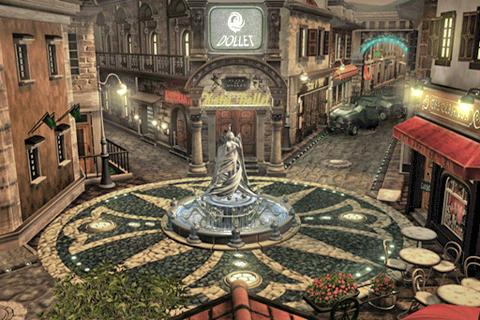
\includegraphics[width=\columnwidth]{./art/siegeofdollet/dollet.jpg} 
%
\vfill
%
Vocês devem chegar logo à praia Lapin, antes de Dollet.
Os Galbadianos construíram algumas defesas na costa, mas elas não devem ser páreo para nossas canhoneiras.
Depois que a praia estiver liberada, o esquadrão B seve deixar o barco e começar a prova.
Eles podem subir as escadarias à esquerda e de lá, seguir o beco até a praça da cidade.
Consigo ver 3 soldados Gabadianos protegendo o centro da cidade, embora possa haver mais.
Cada estudante deve passar num teste de DF~7 para ser capaz de os perceber também.
Vamos ver como eles se viram sozinhos.
%
\vfill
%
\ofmonster{Soldado Galbadiano}{2}{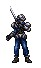
\includegraphics[width=0.15\columnwidth]{./art/siegeofdollet/gsoldier.jpg}}
{
	PV: & \hfill 13 & PM: & \hfill 0\\
	FOR: & \hfill 2 & DEF: & \hfill 1 \\
	MAG: & \hfill 0 & RES: & \hfill 0 \\
	AGI: & \hfill 2 & Tamanho: & \hfill M\\
}
{\accf{Metralhadora}: 1d Dano, 3u Alcance \hfill \accf{Deixa:} 200G}{}
%
\vfill
%
Os Galbadianos com certeza não facilitarão para eles. Pois, estão usando a fonte como cobertura para evitar o confronto físico. Após derrotá-los, o esquadrão B só precisa garantir que o centro da cidade esteja segura.
Se decidirem procurar ao redor, eles podem encontrar alguns itens úteis como poções.
Há também um cachorro solitário perambulando por ali, o pobrezinho provavelmente se perdeu na confusão.
Já faz uma hora e acho que os estudantes estão ficando entediados.
Parece que tudo está... espere um segundo.
Posso ver um grupo grande de Galbadianos se movendo rapidamente em direção à praça da cidade!
O esquadrão B precisa se esconder imediatamente!
Hum... não parece que os soldados querem retomar o centro da cidade, eles estão indo a algum outro lugar.
O que estão tramando?
%
\vfill
%
Eles estão se movendo em direção ao caminho da montanha, mas não há coisa alguma lá, exceto uma velha torre de rádio, eu acho.
Não sei se os estudantes entenderam o que está acontecendo, mas o cachorro sim.
Bem, pelo menos ele está uivando para a montanha.
Quais são as ordens Instrutor?
Lembre-se, o esquadrão B precisa guardar o centro da cidade, mas estes Galbadianos estão aprontando alguma coisa, com certeza.
Espero que os estudantes sigam suas ordens...
%
\clearpage
%
\ofquote{"WEDGE! Onde você está!? Sem pagamento este mês!" }{Major Biggs}
%
\vfill
%
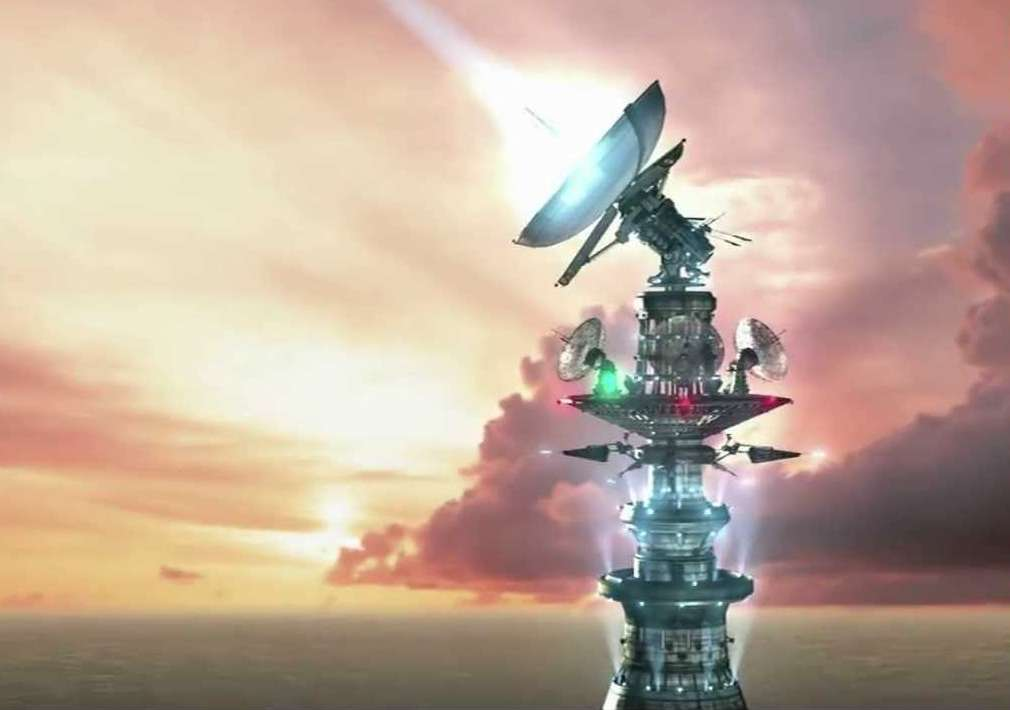
\includegraphics[width=\columnwidth]{./art/siegeofdollet/tower.jpg}
%
\vfill
%
O esquadrão B também está indo para a montanha, espero que eles não sejam detectados. há alguns soldados de Dollet guardando a passagem, mas os Galbadianos estão passando por eles como se fossem de papel.
Mesmo assim, eles sofreram muitas baixas no caminho, acho que somente 2 deles realmente conseguiram chegar à torre.
O esquadrão~B deve ser capaz de alcançar a torre sem problemas. Parece que eles estão quase chegando ao topo da montanha. 
Nesse meio tempo, os Galbadianos alcançaram a plataforma da torre de rádio e acho que estão fazendo reparos. Pelo menos conseguiram reativar a torre de rádio.
Isso significa que os estudantes podem pegar o elevador do térreo até lá em cima.
%
\vfill
%
\ofmonster{Major Biggs}{2}{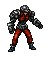
\includegraphics[width=0.22\columnwidth]{./art/siegeofdollet/biggs.jpg}}
{
	PV: & \hfill 28 & PM: & \hfill 24\\
	FOR: & \hfill 2 & DEF: & \hfill 2 \\
	MAG: & \hfill 1 & RES: & \hfill 1 \\
	AGI: & \hfill 2 & Tamanho: & \hfill M\\
}
{\accf{Metralhadora}: 1d Dano, 3u Alcance \hfill \accf{Deixa:} 500G}
{
	\mspell{Raio}{4}{0r}{Único}{3u}{Cause 2d de dano de Raio ao alvo.}{\lightning}	
	\mtech{Rush}{3}{0r}{Único}{Arma}{Ataque o alvo, se acertar, empurre-o 1u para trás além do dano causado.}{}	
}
%
\vfill
%
\ofmonster{Wedge}{2}{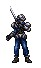
\includegraphics[width=0.15\columnwidth]{./art/siegeofdollet/gsoldier.jpg}}
{
	PV: & \hfill 22 & PM: & \hfill 16\\
	FOR: & \hfill 2 & DEF: & \hfill 1 \\
	MAG: & \hfill 1 & RES: & \hfill 1 \\
	AGI: & \hfill 3 & Tamanho: & \hfill M\\
}
{\accf{Espada}: 1d Dano \hfill \accf{Deixa:} 300G}
{\mspell{Fogo}{4}{0r}{Único}{3u}{Cause 2d de dano de Fogo ao alvo.}{\fire}	}
%
\newpage
Agora eu posso ver o esquadrão B no topo da torre, enfrentando os soldados Galbadianos, um deles parece ser o líder.
Acho que entendi sua estratégia: eles estão tentando forçar os estudantes à borda da plataforma para os derrubar de lá.
Caso isso aconteça, acho que os estudantes deverão ser capazes de se segurar em alguma coisa se passarem num teste de DF 5, ou se um aliado puder usar sua ação para os puxar de volta.
De qualquer forma, os Galbadianos não parecem muito competentes e... o esquadrão B foi capaz de neutralizar o inimigo!
Também acabamos de receber uma ordem importante:
todos os esquadrões devem recuar até a praia Lapin imediatamente, nossos barcos partirão em meia hora.
Os esquadrões que não conseguirem alcançar a costa nesse tempo, serão deixados para trás!
Acho que o esquadrão B pode... espere, mais que Kupo é ISSO?!\\\\
%
\vfill
%
\ofmonster{X-ATM092}{4}{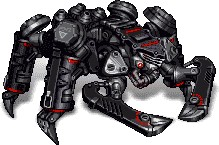
\includegraphics[width=0.3\columnwidth]{./art/siegeofdollet/mech.jpg}}
{
	PV: & \hfill ??? & PM: & \hfill 80\\
	FOR: & \hfill 2 & DEF: & \hfill 3 \\
	MAG: & \hfill 0 & RES: & \hfill 1 \\
	AGI: & \hfill 4 & Tamanho: & \hfill G\\
}
{\accf{Garra}: 2d Dano, 2u Alcance}
{
	\mtech{Feixe explosivo}{5}{0r}{2u}{5u}{Cause 2d de dano de Fogo a todos os inimigos na área.}{\fire}	
	\mtech{Braço esmagador}{3}{0r}{Único}{Arma}{ alvo faz um teste de DF 8 ou sofre 2d de dano e fica Imóvel por 1 rodada.}{\immobile}	
}
%
\vfill
%
Não sei de onde os Galbadianos tiraram essa coisa, mas ela está correndo atrás dos estudantes.
Parece que ela alcançará todos os membros do esquadrão que falharam no teste de DF 8, espero que o resto não os deixem para trás.
Não há jeito do esquadrão B destruir isso em combate, especialmente se eles quiserem chegar à costa à tempo.
Embora, haja outra maneira: se atacarem as pernas daquela coisa algumas vezes, elas colapsarão e iniciará os reparos em si mesma, o que os dará tempo para correr.
É uma das vulnerabilidades comuns conhecidas das máquinas dos Galbadianos, então deve funcionar.
Ainda assim, acho que eles terão de lutar com a coisa pelo menos duas vezes antes de alcançarem a costa.
É possível que pensem em alguma coisa a fim de para aquilo, um bloqueio ou distração talvez?
%
\vfill
%
O esquadrão B está correndo pela Dollet e se aproximando da praia, mas a máquina ainda os seguem.
Instrutor, há uma poderosa metralhadora montada no deque do seu barco, ela deve dar cabo daquilo!
... Acho que conseguiu, ótimo trabalho!
O esquadrão B também embarcou, então vocês estão prontos para partir!
Ufa... essa passou perto, espero que todos tenham conseguido voltar a salvo.
Então, Instrutor, o que achou? Como os estudantes foram na prova? Quais deles devem ser promovidos a SeeD?
%
\clearpage